\documentclass[tikz]{standalone}

% features
% - for loop
% - \pgfdeclareshape
% - \path and intersection
% - \coordinate
% - \brace


\usetikzlibrary{positioning} % easier and more flexible way to position nodes relative to each other. With this library, you can use syntax such as right=of some-node or above left=of another-node to position a node relative to another node.
\usetikzlibrary{shapes} % ellipse
\usetikzlibrary{calc}
\usetikzlibrary{decorations.pathmorphing}
\usetikzlibrary{decorations.pathreplacing}
\usetikzlibrary{intersections}

\makeatletter
\pgfdeclareshape{vshape}{
    % This error occurs because the center anchor is defined by default for all shapes in TikZ, and it is used internally by TikZ to position nodes relative to each other. Therefore, when you remove the center anchor from your custom shape, TikZ no longer knows how to position nodes relative to it. To avoid this error, you should always define the center anchor in your custom shapes, even if you don't plan to use it explicitly.
    \savedanchor\centerpoint{ % center
    \pgf@x=0pt
    \pgf@y=5pt
    }
    \anchor{center}{
        \centerpoint
    }

    \savedanchor\southpoint{ % south
    \pgf@x=0pt
    \pgf@y=0pt
    }
    \anchor{south}{
        \southpoint
    }

    \savedanchor\westpoint{ % west
        \pgf@x=-5pt
        \pgf@y=0pt
    }
    \anchor{west}{
        \westpoint
    }

    \savedanchor\eastpoint{ % east
        \pgf@x=5pt
        \pgf@y=0pt
    }
    \anchor{east}{
        \eastpoint
    }

    \savedanchor\northpoint{ % north
        \pgf@x=0pt
        \pgf@y=10pt
    }
    \anchor{north}{
        \northpoint
    }
    \backgroundpath{
    \pgfpathmoveto{\westpoint}
    \pgfpathlineto{\northpoint}
    \pgfpathlineto{\eastpoint}
    % \pgfpathclose
    \pgfusepath{stroke} % draw the path that has been constructed using the \pgfpath...
    }
}
\makeatother

\newcommand{\plasma}[3]{
    \begin{scope}[shift={(#1)}, transform shape, scale=#2, rotate=#3]
        % Define the control points for the Bezier curves
        \def\cpa{(0,0)}
        \def\cpb{(1,-1)}
        \def\cpc{(2,-0.5)}
        \def\cpd{(2.5,0.5)}
        \def\cpe{(2.5,1.5)}
        \def\cpf{(1.5,2)}
        \def\cpg{(0.5,1)}
        \def\cph{(0,1)}
        
        % Draw the Bezier curves
        \draw[thick] plot [smooth cycle, tension=1] coordinates {\cpa \cpb \cpc \cpd \cpe \cpf \cpg \cph};
        
        % Add some shading to give the rock a 3-D effect
        \shade[top color=blue!50, bottom color=gray!50] plot [smooth cycle, tension=1] coordinates {\cpa \cpb \cpc \cpd \cpe \cpf \cpg \cph};
    \end{scope}
}

\newcommand{\satellite}[4]{% #1 = x-coordinate, #2 = y-coordinate, #3 = scale, #4 = rotate
  \begin{scope}[shift={(#1,#2)}, transform shape, scale=#3, rotate=#4] %  transform shape option ensures that the transformations are applied to the nodes within the scope, rather than just to the scope itself.
    % central part
    \node[draw, black, name=central-part] at (0,0) [minimum size=1cm] {};
    
    % right little square
    \node[draw, shape=rectangle, name=right-little-square, minimum size=0.3cm, right=0cm of central-part, anchor=west] {};

    % right photovoltaic
    \node[draw, shape=rectangle, name=right-photovoltaic, minimum height=1cm, minimum width=2cm, right=0cm of right-little-square, anchor=west] {};
    
    % right left square
    \node[draw, shape=rectangle, name=left-little-square, minimum size=0.3cm, left=0cm of central-part, anchor=east] {};

    % left photovoltaic
    \node[draw, shape=rectangle, name=left-photovoltaic, minimum height=1cm, minimum width=2cm, left=0cm of left-little-square, anchor=east] {};

    % antenna
    \node[draw, name=antenna-base, shape=ellipse, minimum width=2cm, minimum height=.5cm, below=0cm of central-part] {};
    \node[draw, name=antenna-sat, shape=isosceles triangle, isosceles triangle apex angle=60, shape border rotate=90, minimum height=0.5cm, inner sep=0pt, below=0cm of antenna-base.center, anchor=south, rotate=180] {};

  \end{scope}
}

\begin{document}
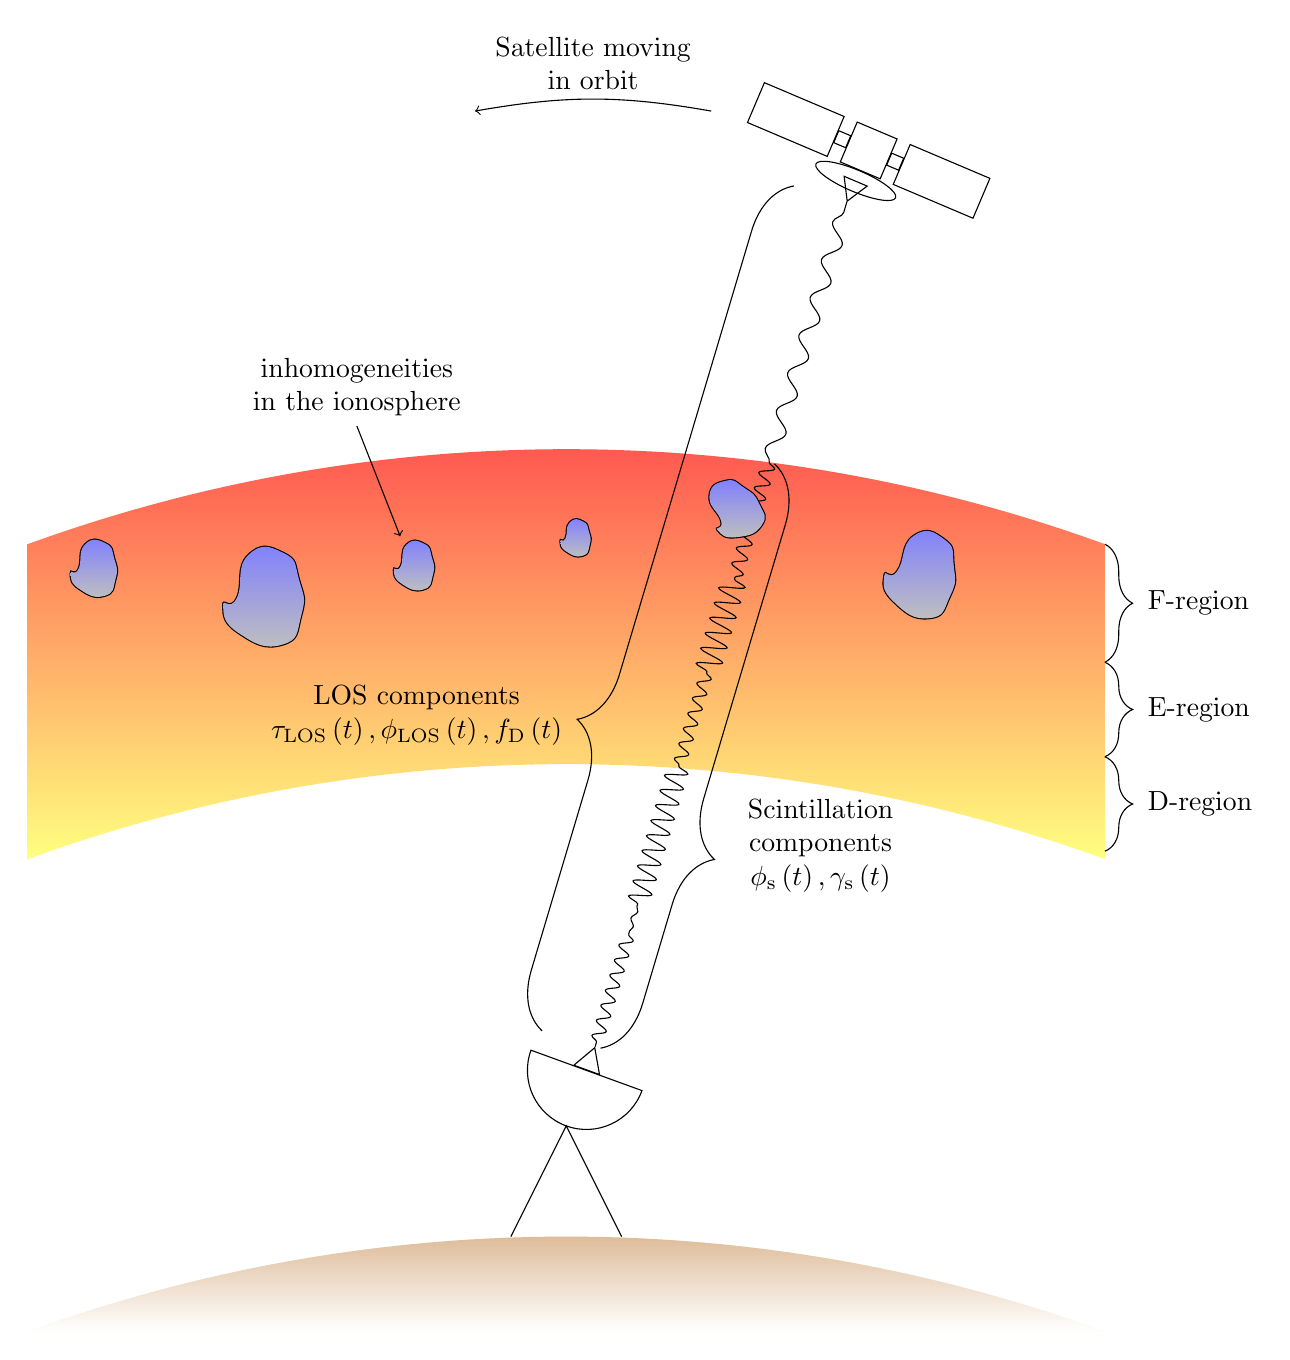
\begin{tikzpicture}
    %% Earth
    %% draw an arc and save the coordinate of its top
    \shade[top color=brown!70, very thick,fill=yellow!20] (0,0) arc (70:110:20cm) coordinate[pos=0.5] (top); % (<init-degree>:<final-degree>:<radius>)
    %% uncomment the line below to see the coordinate that it was saved
    % \draw[red, ultra thick, shift=(top)] (-.1,-.1) -- (.1,.1) (-.1,.1) -- (.1,-.1);

    %% ionosphere
    \shade[top color=red!70, bottom color=yellow!50] (0,10) arc (70:110:20cm)
    coordinate[pos=0] (ionosphere-northeast)
    coordinate[pos=1] (ionosphere-northwest)
    coordinate[pos=0.2,shift={(0,-1.5)}] (ionosphere-plasma1)
    coordinate[pos=0.345,shift={(0,-1)}] (ionosphere-plasma2)
    coordinate[pos=0.5,shift={(0,-1.3)}] (ionosphere-plasma3)
    coordinate[pos=0.65,shift={(0,-1.6)}] (ionosphere-plasma4)
    coordinate[pos=0.8,shift={(0,-1.9)}] (ionosphere-plasma5)
    coordinate[pos=0.95,shift={(0,-0.8)}] (ionosphere-plasma6)
    -- ++(0,-4) arc (110:70:20cm) -- cycle; % -- cycle is used to connect the end of the last path segment with the beginning of the first path segment. second arc is specified using ++ notation, which means that the endpoint of the arc is calculated relative to the current position. using + notation, which means that the endpoint of the arc is calculated relative to the start of the arc.

    %% satellite
    \satellite{-3}{15}{0.55}{-23}
    \draw[->] (-5.0,15.5) to[in=10, out=170] node[above, pos=0.5,align=center] {Satellite moving\\in orbit} (-8.0,15.5);
    % \draw[red, ultra thick, shift=(sat.north)] (-.1,-.1) -- (.1,.1) (-.1,.1) -- (.1,-.1);

    %% receiver
    \node[shape=vshape,fill=blue,minimum width=1cm,minimum height=1cm, below=0cm of top, anchor=south, scale=4] (my-base) {};
    %% to see the anchor positions, uncomment the lines below
    % \foreach \anchor/\shift in {center/below, south/below, north/above, east/right, west/left}
    % \draw [draw=red, shift=(v.\anchor)] node [\shift] {\anchor}
    %     (-.1,-.1) -- (.1,.1) (-.1,.1) -- (.1,-.1);
    
    
    \pgfmathsetmacro{\angle}{-20} % angle rotation
    \draw[rotate=\angle, shift=(my-base.north)] (-0.75,0.75)  arc (-180:0:0.75cm) -- cycle;
    \coordinate (begin) at (my-base.north)+(-0.75,0.75);
    \coordinate (center) at ($(begin) + ({\angle+90}:0.75cm)$); % center point of the half-circle
    \node[draw, shape=isosceles triangle, isosceles triangle apex angle=60, shape border rotate=90, minimum height=0.3cm, inner sep=0pt, below=0cm of center, anchor=south, rotate=\angle] (antenna-receiver) {};

    %% Define the amplitude function
    \pgfmathdeclarefunction{amplitudefunc}{1}{%
    \pgfmathparse{sin(#1*180)/2 + 1}%
    }

    
    %% Find the intersection point between the radio signal and the upper layer of the ionosphere
    \path[name path=upper-arc] (0,10) arc (70:110:20cm); % upper arc of the ionophere layer
    \path[name path=line] (antenna-receiver.north) -- (antenna-sat.north); % radio signal path
    \path[name intersections={of=upper-arc and line, by=upper-intersection}];
    
    %% radio signal
    \draw[decorate, decoration={snake, amplitude=1mm, segment length=5mm}] (upper-intersection) -- (antenna-sat.north); % sat-upper layer of the ionosphere
    \coordinate (initcoordinate) at (upper-intersection); % assign initcoordinate to intersect
    \foreach \i/\amplitude in {0.2/0.9, 0.2/1.6, 0.25/0.8, 0.5/1.4, 0.2/0.3}{ % the "/" works like zip() function in Python
        \coordinate (finalcoordinate) at ($(initcoordinate)!\i!(antenna-receiver.north)$); % applying the draw by parts
        \draw[decorate, decoration={snake, amplitude={\amplitude mm}, segment length=2mm}] (initcoordinate) -- (finalcoordinate);
        \coordinate (initcoordinate) at (finalcoordinate); % assign initcoordinate to finalcoordinate
    }
    \draw[decorate, decoration={snake, amplitude={0.8mm}, segment length=2mm}] (initcoordinate) -- (antenna-receiver.north); % final path


    %% plasmas
    \plasma{ionosphere-plasma1}{0.35}{20}
    \plasma{ionosphere-plasma2}{0.25}{70}
    \plasma{ionosphere-plasma3}{0.15}{30}
    \plasma{ionosphere-plasma4}{0.2}{30}
    \plasma{ionosphere-plasma5}{0.4}{30}
    \plasma{ionosphere-plasma6}{0.23}{30}

    %% regions
    \draw[decorate, decoration={brace, amplitude=10pt}] ({ionosphere-northeast}) -- +(0,-1.5)
    coordinate (init-base)
    node[midway, right=12pt] {F-region};
    \draw[decorate, decoration={brace, amplitude=10pt}] ({init-base}) -- +(0,-1.2)
    coordinate (init-base)
    node[midway, right=12pt] {E-region};
    \draw[decorate, decoration={brace, amplitude=10pt}] ({init-base}) -- +(0,-1.2)
    coordinate (init-base)
    node[midway, right=12pt] {D-region};


    %% LOS components
    \draw[decorate, decoration={brace, amplitude=20pt, raise=20pt, aspect=0.35pt}] (antenna-receiver.north) -- node[xshift=-110pt, yshift=-33pt, align=center] {LOS components\\\(\tau_{\mathrm{LOS}} \left( t \right),\phi_{\mathrm{LOS}} \left( t \right),f_{\mathrm{D}} \left( t \right)\)} (antenna-sat.north);

    %% Find the intersection point between the radio signal and the lower layer of the ionosphere
    \path[name path=lower-arc] (0,10)++(0,-4) arc (70:110:20cm); % lower arc of the ionosphere layer
    \path[name intersections={of=lower-arc and line, by=lower-intersection}];

    %% ionosphere components
    \draw[decorate, decoration={brace, amplitude=20pt, raise=2pt, aspect=0.65pt}] (upper-intersection) --  node[xshift=50pt, yshift=-33pt, align=center] {Scintillation\\components\\\(\phi_{\mathrm{s}} \left( t \right),\gamma_{\mathrm{s}} \left( t \right)\)} (antenna-receiver.north); % lower-intersection

    %% ionosphere inhomogeneities
    \draw[->] (-9.5,11.5) -- (-8.95,10.1) node[pos=0, above, align=center] {inhomogeneities\\in the ionosphere};
    
    
\end{tikzpicture}
\end{document}